\section{Returned Visual Survey: Protocol and Complete Counts}
\label{app:human}

\paragraph{Version and evidence.}
This model-focused presentation retains both originally collected arms and
all eligibility rules; no responses or unfavorable internal-control outcomes
are removed. The per-model pooled summary was added after collection.
This analysis uses the seven-page, all-English visual packets V01--V11,
released September 22, 2026, and the returned archive supplied on GitHub before
this revision. It supersedes the text-based prospective evaluation in earlier
manuscripts; older Q/S/P instruments are not pooled with these responses.
Each coded return has six comparisons and eighteen answers. The source PDF
form values are checked against the selected widget appearance states before
decoding through the frozen allocation. No answers are inferred from a model,
imputed, or edited. The filled Excel file preserves every return, with V04
marked for cover verification and omitted from all preference summaries.

\paragraph{Visual sampling.}
The image arm uses the one archived premise with complete matching render
assets: a cliffside city that taxes spoken promises by weight. Each of seven
world configurations contributes its unaltered map and the first idle-down
frame of its first two requested characters, under the same framing rule.
These are finalized pipeline assets, including recorded repair steps, not
independent fresh generations. The unavailable Luna artifact is not replaced
or counted as a preference loss. Terra's unavailable third publishable
character is not shown; no condition is judged on a third character. This
instrument does not evaluate asset completeness, animation, or navigation.

\paragraph{Structure sampling and presentation.}
The ten matched requests use the fixed first archived replicate of full
Agora and single-pass generation. The diagrams include all source rooms in
source order, count inhabitants by their recorded home location, and show
the count of large scene components with the first component label as an
example. Lines denote containment, not adjacency. The same short English
scene description appears on both sides. The comparison retains readable
source records even when an objective completion contract fails. There are
no matched baseline renderings: no unrelated or synthetic image is substituted.
The conditions retain unequal total generation budgets.

\paragraph{Allocation and masking.}
Seed 20260922 fixes the schedule before response analysis. Every participant
sees four distinct image pairs and two distinct structure pairs. The original
plan has 44 image and 22 structure comparisons; each exact pair occurs twice,
with one seed-selected pair per arm occurring four times. Every pair has
balanced A/B orientation, and Agora appears on A once and B once for each
participant. Excluding V04 removes four image and two structure comparisons,
leaving the coverage counts reported in Section~\ref{sec:human-results}.
Individual pair orientation is consequently no longer universally balanced.
The twenty retained structure comparisons remain balanced overall: Agora is
shown on each side ten times. The questionnaire hides source names, but
visible artifacts can still reveal stylistic clues; analyst blinding is
not claimed.

\paragraph{Questions and estimands.}
Q1 in both arms asks, ``Which world would you rather explore?'' Image Q2 asks
which map is easiest to read; Q3 asks which characters fit their world better.
Structure Q2 asks which world is easiest to understand; Q3 asks which places
fit the scene better. All offer A, B, Same, and Not sure. Exploration measures
\emph{stated interest from the supplied evidence}, not enjoyment after playing.
The diagnostic items measure different constructs across the arms and are
never merged. This explicit separation follows the reporting concerns of
\citet{howcroft}.

Let $w_{jq},t_{jq},\ell_{jq}$ denote Agora wins, ties, and baseline wins for
request $j$ and item $q$, after eligibility filtering. With abstentions excluded,
\begin{equation}
\hat p_{jq}=\frac{w_{jq}+t_{jq}/2}{w_{jq}+t_{jq}+\ell_{jq}},
\qquad \hat p_q=\frac{1}{10}\sum_{j=1}^{10}\hat p_{jq}.
\end{equation}
The ten-request mean is shown only if all ten denominators are nonzero. All
three items meet this condition. Pooled vote scores, provided only as a
weighting diagnostic, are 35.0\%, 42.5\%, and 36.8\%, versus equal-request
scores of 40.0\%, 32.5\%, and 37.5\%. Clockwork has four votes and is preferred
for clarity but not exploration; reporting the estimator explicitly prevents
this imbalance from silently changing the result. Image scores use the same
tie and abstention rule separately within each exact model pair, with no
cross-prompt or global model ranking.

\paragraph{Eligibility, consent, and missing administration records.}
Ten covers affirm age 18 or older, English comprehension, voluntary
participation, and no prior work on the system or exposure to detailed
results. V04 has eighteen choices but no cover answers; blank checkboxes are
treated as unconfirmed, not as an affirmative response or a known refusal.
The exclusion rule was included in the original release and does not depend
on preferred source. The archive supplies no names or demographics beyond
the cover confirmations, nor independent verification that codes correspond
to distinct people. The organizer reports online volunteer recruitment with no compensation,
and identifies V04 as an accidentally omitted cover. This explanation does
not supply the missing participant confirmations. No sampling frame or
probability-sampling procedure is documented; recruitment is treated as an
online volunteer sample. Actual completion time and an ethics approval or
exemption record were not supplied. No approval, exemption, representative
sampling, or measured 10--15-minute completion time is claimed.

\paragraph{Response dependence and presentation checks.}
The 180 item responses come from ten coded returns; they are not 180
independent people. All image comparisons reuse seven artifacts on one scene,
and all three questions reuse each displayed pair. We report counts and
request-level variation, without item-level significance tests, Elo scores,
or confidence intervals that would imply unsupported population precision.
Image Q1 selects A 15 times and B 25 times; structure Q1 selects A 11 times
and B 9 times. This descriptive side asymmetry is retained for inspection,
but does not identify a position effect separately from artifact preference.
No respondent is excluded for a repeated choice pattern or for favoring the
baseline. Very small per-pair counts make agreement coefficients unstable;
the full counts are reported instead.

\begin{table*}[t]
\centering\small
\setlength{\tabcolsep}{5pt}
\begin{tabularx}{\textwidth}{@{}Yrrr@{}}
\toprule
Request & Explore & Clarity & Scene fit \\
\midrule
Archive Of Borrowed Gravity & 50\% (1/0/1/0) & 25\% (0/1/1/0) & 50\% (1/0/1/0) \\
Aurora Court Of Migrating Cities & 50\% (1/0/1/0) & 100\% (2/0/0/0) & 100\% (2/0/0/0) \\
Cartographer Lung Exchange & 0\% (0/0/1/0) & 0\% (0/0/1/0) & 0\% (0/0/1/0) \\
Clockwork Rain Conservatory & 0\% (0/0/4/0) & 100\% (4/0/0/0) & 25\% (1/0/3/0) \\
Intertidal Embassy For Extinct Rivers & 0\% (0/0/2/0) & 0\% (0/0/2/0) & 0\% (0/0/2/0) \\
Museum Of Future Debts & 0\% (0/0/2/0) & 0\% (0/0/2/0) & 0\% (0/0/2/0) \\
Mycelium Patent Bazaar & 100\% (1/0/0/0) & 0\% (0/0/1/0) & 0\% (0/0/1/0) \\
Night Market Of Unfinished Weather & 50\% (1/0/1/0) & 50\% (1/0/1/0) & 50\% (1/0/1/0) \\
Sunken Satellite Monastery & 50\% (1/0/1/0) & 0\% (0/0/2/0) & 50\% (1/0/1/0) \\
Tidal Embassy Of Lost Languages & 100\% (2/0/0/0) & 50\% (1/0/1/0) & 100\% (1/0/0/1) \\
\bottomrule
\end{tabularx}

\caption{Every structure request. Each cell gives the Agora preference score
and counts (Agora wins / ties / baseline wins / Not sure). The requests,
not the number of ratings, are equally weighted in the main result.}
\label{tab:human-structure-detail}
\end{table*}

\begin{table}[t]
\centering\small
\setlength{\tabcolsep}{5pt}
\begin{tabular}{@{}lrrr@{}}
\toprule
Pair & Explore & Map & Characters \\
\midrule
M1--M2 & 2/0/0/0 & 2/0/0/0 & 1/0/0/1 \\
M1--M3 & 1/0/0/0 & 0/0/1/0 & 1/0/0/0 \\
M1--M4 & 2/0/0/0 & 2/0/0/0 & 2/0/0/0 \\
M1--M5 & 1/0/0/0 & 1/0/0/0 & 1/0/0/0 \\
M1--M6 & 1/0/1/0 & 1/0/1/0 & 1/0/1/0 \\
M1--M7 & 1/0/1/0 & 1/0/1/0 & 1/0/1/0 \\
M2--M3 & 1/0/1/0 & 0/1/1/0 & 1/0/1/0 \\
M2--M4 & 2/0/0/0 & 0/0/2/0 & 1/0/1/0 \\
M2--M5 & 2/0/0/0 & 0/0/2/0 & 1/0/1/0 \\
M2--M6 & 1/0/0/0 & 0/0/1/0 & 1/0/0/0 \\
M2--M7 & 0/0/1/0 & 0/0/1/0 & 0/0/1/0 \\
M3--M4 & 1/0/1/0 & 2/0/0/0 & 1/1/0/0 \\
M3--M5 & 0/0/2/0 & 0/0/2/0 & 1/0/1/0 \\
M3--M6 & 0/0/2/0 & 0/0/2/0 & 0/0/2/0 \\
M3--M7 & 0/0/2/0 & 0/0/2/0 & 0/0/1/1 \\
M4--M5 & 1/0/1/0 & 0/0/2/0 & 1/0/1/0 \\
M4--M6 & 2/0/0/0 & 0/0/2/0 & 2/0/0/0 \\
M4--M7 & 2/0/2/0 & 0/0/4/0 & 2/0/2/0 \\
M5--M6 & 2/0/0/0 & 0/0/2/0 & 2/0/0/0 \\
M5--M7 & 0/0/2/0 & 0/0/2/0 & 0/0/2/0 \\
M6--M7 & 1/0/1/0 & 1/0/1/0 & 2/0/0/0 \\
\bottomrule
\end{tabular}

\caption{Every image pair. Entries are first-source wins / ties /
second-source wins / Not sure. Each row describes the same pair under three
different questions; these are not independent respondent samples.}
\label{tab:human-image-detail}
\end{table}

\paragraph{Image identity key.}
M1: Gemini 2.5 Flash; M2: Gemini 3.1 Flash Lite; M3: Gemini 3.1 Pro Preview; M4: Gemini 3.5 Flash Lite; M5: Gemini 3.7 Flash; M6: GPT-5.6 Sol; M7: GPT-5.6 Terra.

These names preserve archived backend identifiers and do not independently
verify product naming, an immutable provider snapshot, or common inference
budgets. The actual visual artifacts, rather than the labels, are the measured
objects.

\subsection{Internal Generation Procedure Control}
\label{app:internal-generation}
This supplementary comparison varies the generation procedure within the
Agora implementation. Both conditions use its world representation and
rendering conventions; they are not independent world-generation systems.
The total generation budgets also differ, so this is a procedure control,
not a compute-matched component ablation. The returned results below are
retained in full and must not be interpreted as Agora's performance against
an external system.
For each item, a preference for Agora scores 1, a tie 0.5, and a baseline
preference 0; ``Not sure'' is excluded from that item's preference denominator
and reported separately. We average within each request and then equally
across all ten requests, as specified in the released workbook. This prevents
the request receiving four ratings from dominating the overall estimate.

\begin{table}[t]
\centering\small
\setlength{\tabcolsep}{3.2pt}
\begin{tabularx}{\columnwidth}{@{}Yrrrrr@{}}
\toprule
Item & Full & Base & Tie & ? & Score \\
\midrule
Explore & 7 & 13 & 0 & 0 & 40.0\% \\
Clarity & 8 & 11 & 1 & 0 & 32.5\% \\
Scene fit & 7 & 12 & 0 & 1 & 37.5\% \\
\bottomrule
\end{tabularx}

\caption{Structure judgments from ten eligible returns. Full and Base denote Agora
and the single-pass baseline, irrespective of randomized A/B labels; ? = Not
sure. Counts pool twenty comparisons per item. Score is Agora's
\emph{equal-request} mean, not a pooled vote fraction.
No population superiority is inferred from these small counts.}
\label{tab:human-structure}
\end{table}

Respondents select the baseline in thirteen of twenty exploration choices,
versus seven for Agora. Agora's equal-request preference is 40.0\% for
exploration, 32.5\% for world clarity, and 37.5\% for place--scene fit
(Table~\ref{tab:human-structure}). These observations favor the single-pass condition on the displayed
containment diagrams. They neither benchmark Agora against a separate system
nor measure the contribution of its shared representation, renderer, or
runtime. A causal claim about decomposition would additionally require
equalized budgets and controlled retries.

The pattern varies by request (Figure~\ref{fig:human-structure}). Both Tidal
raters prefer Agora for exploration. All four Clockwork raters prefer the
baseline for exploration while choosing Agora for clarity. Understandability
and desire to explore are thus distinguishable judgments in these returns;
we do not sum them into a single quality score. One or two raters on most
requests cannot identify why a design was preferred, and the diagram omits
institutions, social behavior, and actual play. Equal-compute generation and
interactive evaluation remain separate open tests.

\begin{figure*}[t]
\centering
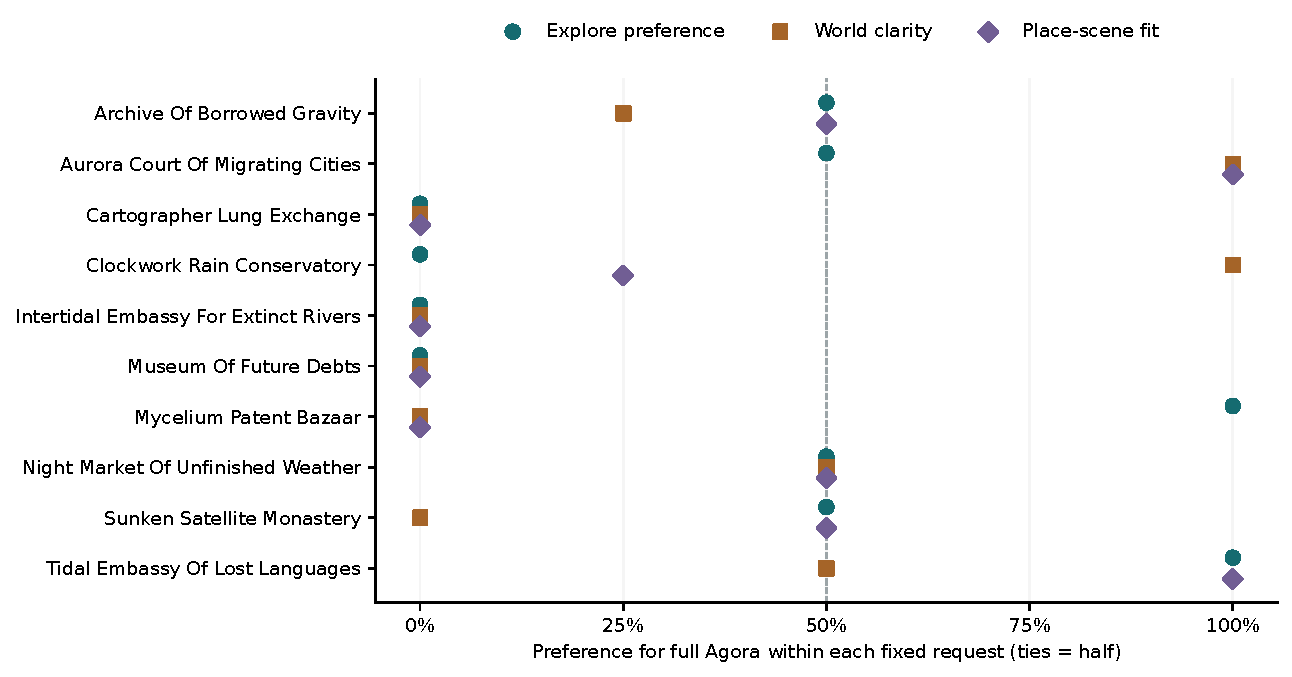
\includegraphics[width=\textwidth]{figures/human_structure_preferences.pdf}
\caption{\paneltitle{World structure: preferences vary by request and item.}
Each point is the fraction favoring full Agora for one request and question,
with a half vote for a tie. The analysis includes 20 comparisons: seven
requests have two raters, two have one, and Clockwork has four. For Tidal
scene fit, one of two raters selects Not sure. These are descriptive fixed-
artifact scores; the dashed line marks equal preference, not a significance
threshold.}
\label{fig:human-structure}
\end{figure*}

